\section{Représentation des données}
\setcounter{exemple}{1}

\subsection{Représentation graphique : diagramme en barres}
\begin{definitionbox}
    Un \hlb{diagramme en barres} (aussi appelé \hlb{diagramme en bâtons}) est un
    graphique qui à chaque valeur, associe un bâton (segment) de
    \bb{hauteur proportionnelle} à l'effectif correspondant.
\end{definitionbox}

\begin{center}
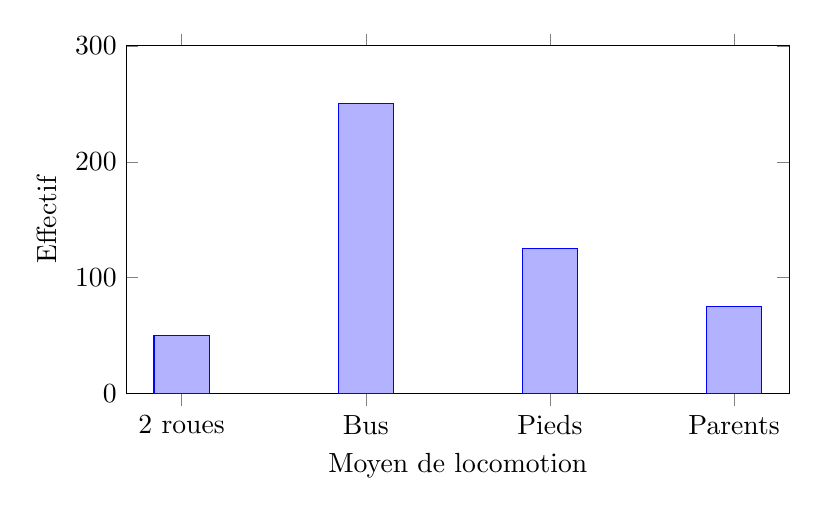
\begin{tikzpicture}
\begin{axis}[
    ybar,
    xlabel={Moyen de locomotion},
    ylabel={Effectif},
    ymin=0,
    ymax=300,
    xtick={1,2,3,4},
    xticklabels={2 roues,Bus,Pieds,Parents},
    bar width=20pt,
    width=10cm,
    height=6cm,
]
\addplot coordinates {
    (1,50)
    (2,250)
    (3,125)
    (4,75)};
\end{axis}
\end{tikzpicture}
\end{center}

\begin{aretenir}
    La hauteur des barres est \bb{proportionnelle} aux effectifs.
\end{aretenir}


\subsection{Représentation graphique : diagramme circulaire}
\begin{definitionbox}
    Un \hlb{diagramme circulaire} (aussi appelé \hlb{diagramme en camembert}) est un
    graphique qui à chaque valeur, associe un 
    \answer{secteur d'angle} proportionnel à l'effectif correspondant. \\
\end{definitionbox}
\begin{methodebox}
    Pour calculer la mesure de l'angle de chaque secteur, on utilise un \bb{tableau
    de proportionnalité} entre la fréquence en pourcentage et l'angle en degrés 
    (\it{le coefficient de proportionnalité est alors de 3.6})

    \begin{center}
    \begin{tabular}{|l|c|c|c|c|c|}
        \hline

       \bb{Transport} & \bb{2 roues} & \bb{Bus} & \bb{À pied} & \bb{Parents} & \bb{Total}\\

       \hline
       \bb{Fréquences en \%} & 10\% & 50\% & 25\% & 15\% & 100\% \\
        \hline
       \bb{Mesure de l'angle en degrès} & \answer{$36$} & \answer{$30$} &
        \answer{$90$} & \answer{$75$} & \answer{$360$} \\
        \hline
    \end{tabular}
    \end{center}

\end{methodebox}
\begin{exempleboxsuite}
    Toujours dans le cas de notre premier exemple, le diagramme circulaire de la
    répartition des élèves selon leur moyen de locomotion est : 
    \begin{center}
    \begin{tikzpicture}
    \pie{
        10/Deux roues,
        50/Bus,
        25/À pied,
        15/Parents
    }
    \end{tikzpicture}
    \end{center}

\end{exempleboxsuite}

\begin{aretenir}
    Les angles des secteurs sont \bb{proportionnels} aux effectifs.
\end{aretenir}


% \subsection{Pourquoi utiliser des représentations graphiques différentes ?}
% \begin{remarquebox}
%     En fonction des données que l'on souhaite analyser, de l'information
%     que l'on souhaite extraire, il peut être plus judicieux d'utiliser un
%     diagramme plutôt qu'un autre. \\
% 
%     Le domaine des statistiques est l'un des domaines les plus riches de
%     mathématiques et trouve de nombreuses applications dans le quotidien. Il est
%     utilisé par les scientifiques, \bb{mais pas que !} \\
% 
%     En effet, au cours de ta vie tu feras face à de nombreuses situations où il
%     te faudra analyser des statistiques. A toi de savoir comment les représenter
%     pour comprendre l'information. \\
% 
%     Prenons notre exemple précédent.
% \end{remarquebox}
% 
% \begin{exempleboxsuite}
%     Si je souhaite connaitre le \bb{nombre} d'élèves venant au collège à pied,
%     autrement dit \answer{l'effectif} des élèves venant au collège à pied, il
%     vaut mieux utiliser \answer{un diagramme à barres} ou un \answer{tableau des
%     effectifs}. En effet il nous
%     donne \bb{directement} accès à cette information ! C'est beaucoup plus compliqué
%     en utilant un \answer{diagramme circulaire}. \\
% 
%     En revanche si je souhaite connaître la \bb{proportion} d'élève venant à
%     pied, autrement dit la \answer{fréquence} des élèves venant à pied, il est plus
%     judicieux d'utiliser un \answer{diagramme circulaire}. En effet il nous
%     donne \bb{directement} accès à cette information ! C'est beaucoup plus compliqué
%     en utilant un \answer{diagramme à bâtons}. \\
% \end{exempleboxsuite}
